% !TEX program = xelatex
\documentclass[UTF8,a4paper,oneside,openany,zihao=5,fontset=none]{ctexrep}

% 本文件集中维护封面和 PDF 元数据，避免多个入口出现信息漂移。
\newcommand{\ReportTitle}{CoTriage：面向工业多设备日志的\\云边协同智能故障感知与决策系统}
\newcommand{\ReportShortTitle}{CoTriage 云边协同智能故障感知与决策系统}
\newcommand{\ReportSubtitle}{挑战杯作品报告}
\newcommand{\ReportTopic}{XH-202606 面向云边协同场景的分布式人工智能感知与决策关键技术研究}
\newcommand{\ReportTeam}{CoTriage 项目组}
\newcommand{\ReportOrganization}{学校／单位信息待提交前补充}
\newcommand{\ReportVersion}{}
\newcommand{\ReportDate}{2026 年 8 月}
\newcommand{\ReportEntryCode}{593751}
\newcommand{\ReportCompetition}{2026年度中国青年科技创新“揭榜挂帅”擂台赛}
\newcommand{\ReportTrack}{学生赛道}
\newcommand{\ReportSchool}{华南师范大学}
\newcommand{\ReportSponsor}{山东浪潮数据库技术有限公司}
\newcommand{\ReportEntryTitle}{面向工业场景的云边协同实时日志分诊告警系统 CoTriage}
\newcommand{\ReportAdvisor}{李杰、李若梅}
\newcommand{\ReportMembers}{庞健、缪招涛、林敬舒、吴侯、钟艺、高成飞、吴佑骏、叶永亮、吴允澎、陈俊杰}

\usepackage{cotriage-report}
\usepackage[
  backend=biber,
  style=gb7714-2015,
  gbnamefmt=familyahead,
  sorting=none
]{biblatex}
\addbibresource{references.bib}

\begin{document}
\hypersetup{pageanchor=false}
\MakeCoTriageCover
\hypersetup{pageanchor=true}
\pagenumbering{Roman}
\MakeCapabilityOverview
\begingroup
\small
\tableofcontents
\endgroup
\clearpage

\pagenumbering{arabic}
\chapter{版式样张}
\section{正文、图与引用}
CoTriage 将连续日志组织为“多节点采集—边缘分层推理—动态路由—云端诊断—反馈写回”的事件链。Redis Streams 提供持续事件传递基础\cite{redisstreams}，Kubernetes 支撑组件部署与扩展\cite{kubernetes}。

\begin{figure}[htbp]
  \centering
  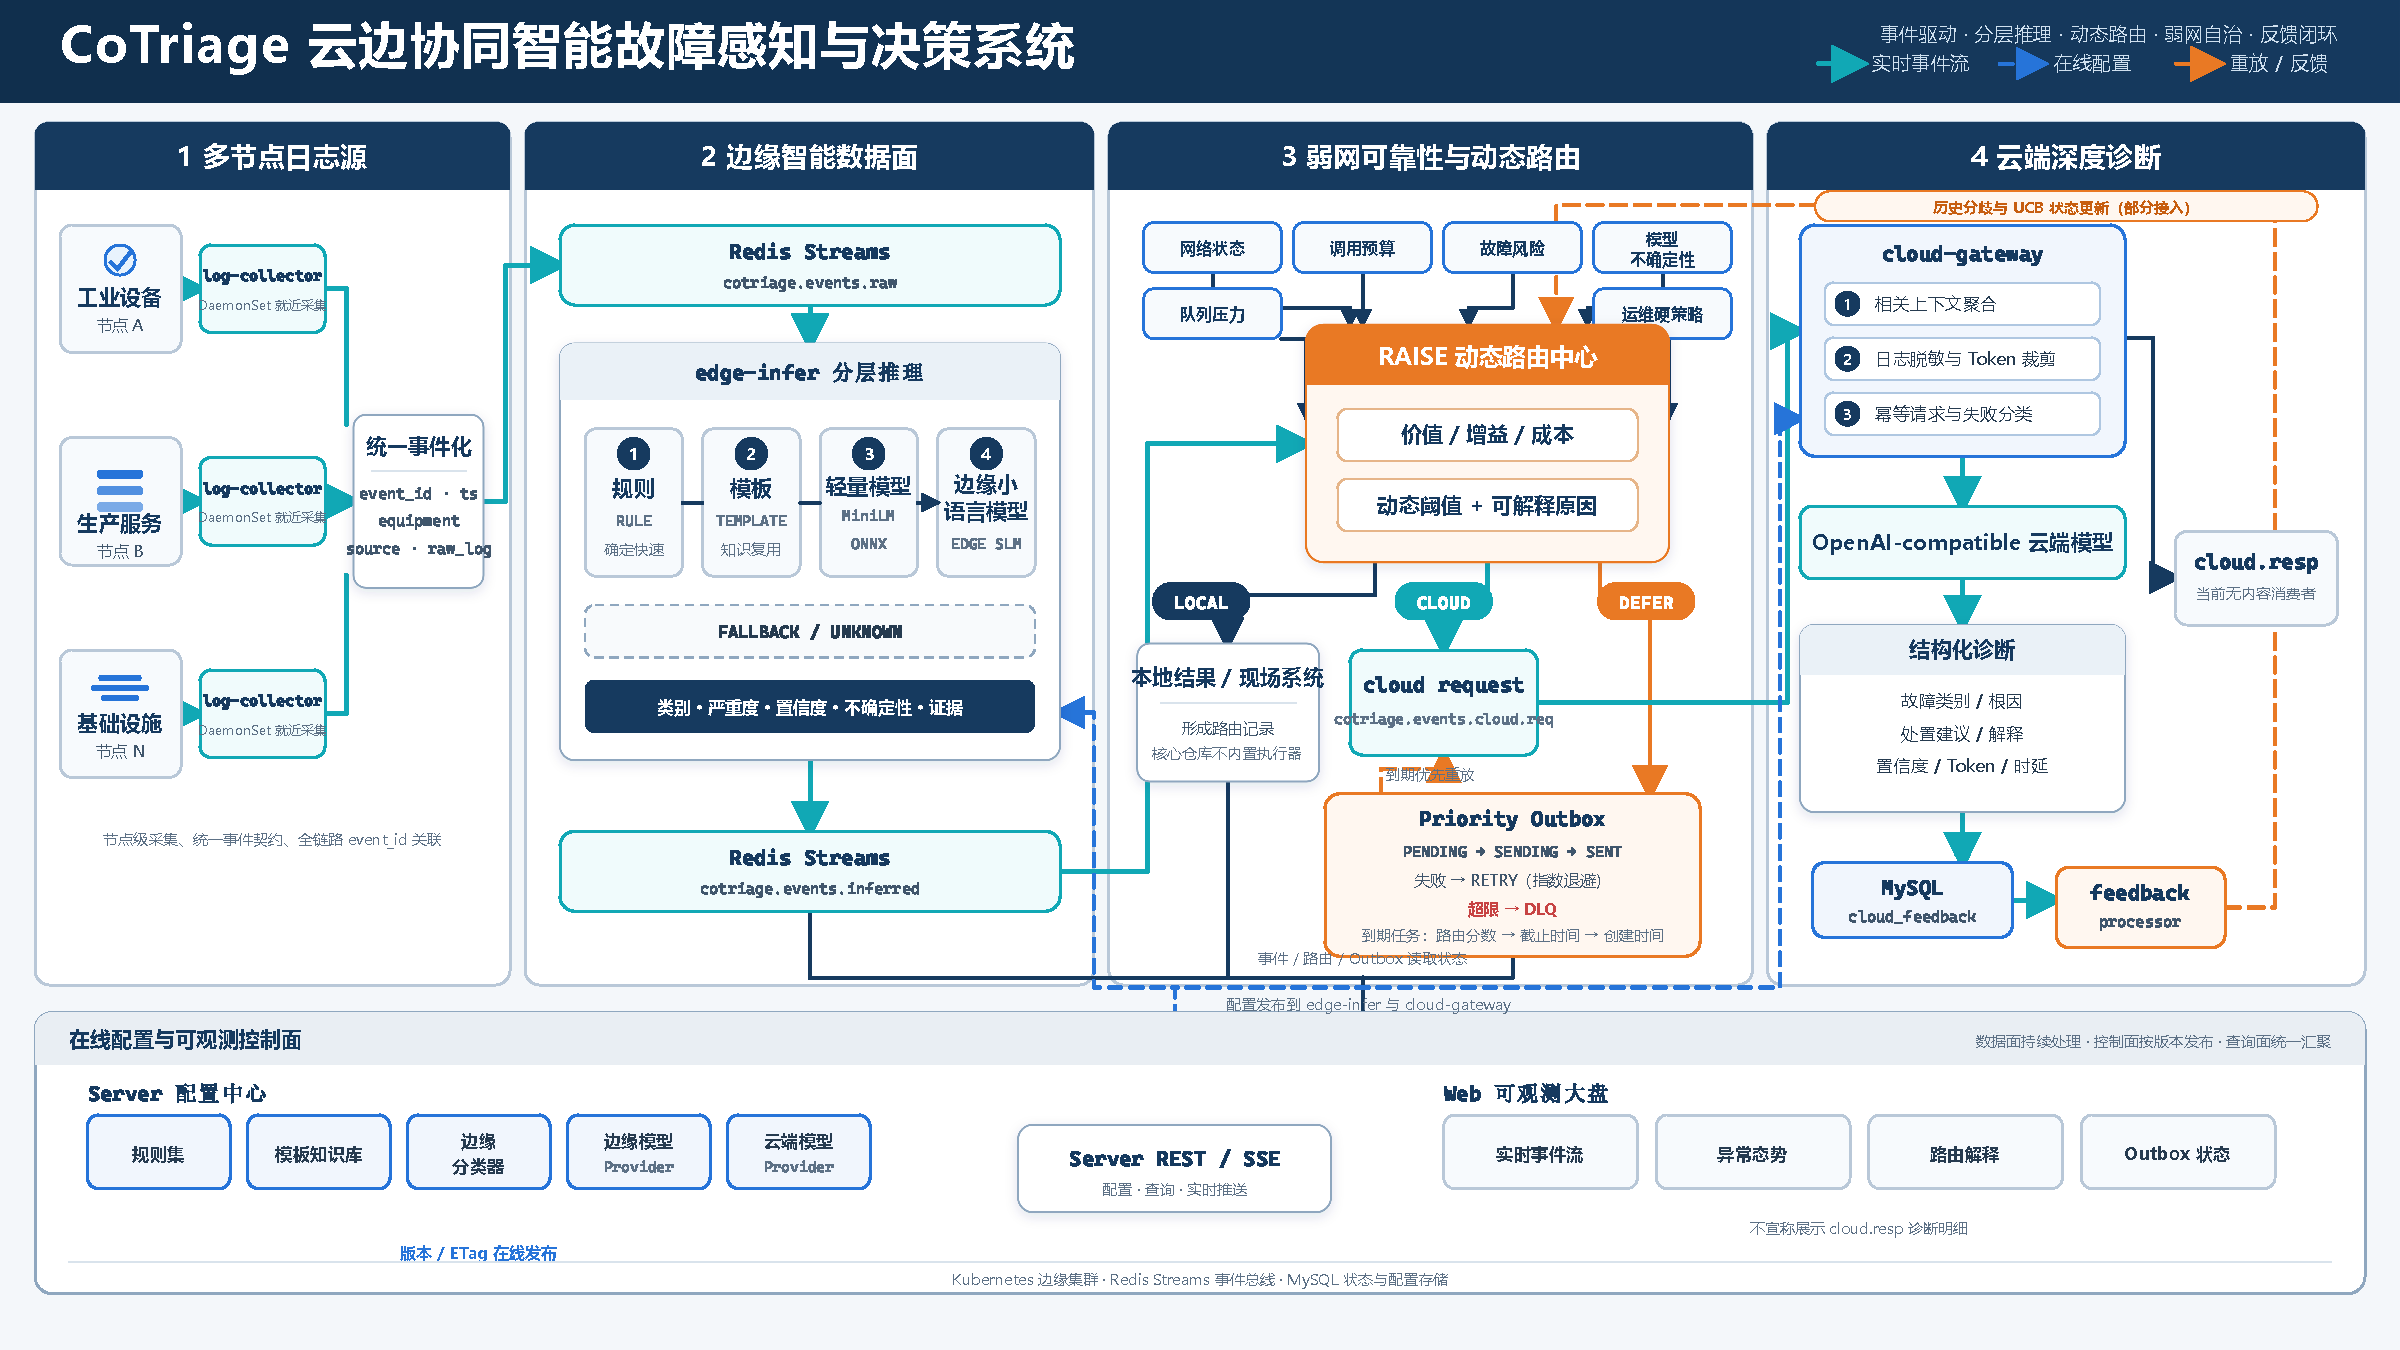
\includegraphics[width=\textwidth]{figures/cotriage-system-architecture.pdf}
  \caption{矢量架构图样张}
\end{figure}

\section{公式与算法}
\begin{equation}
S_t=\beta_vV(e_t)+\beta_gG(e_t)-\beta_kK(e_t,s_t).
\end{equation}

\begin{algorithm}[htbp]
  \caption{三动作路由版式样张}
  \KwInput{事件、边缘结果、系统状态与运维策略}
  \KwOutput{\texttt{LOCAL}、\texttt{CLOUD} 或 \texttt{DEFER}}
  执行硬策略并计算事件分数与动态门槛\;
  根据发送条件输出动作并保存解释\;
\end{algorithm}

\section{宽表与运行截图}
\begin{table}[htbp]
  \centering
  \footnotesize
  \caption{赛题口径与当前运行页面字段的对应关系}
  \label{tab:metric-interpretation}
  \begin{tabularx}{\textwidth}{>{\bfseries\raggedright\arraybackslash}p{0.15\textwidth} p{0.22\textwidth} p{0.23\textwidth} X}
    \toprule
    指标方向 & 赛题口径 & 当前页面显示 & 解释说明 \\
    \midrule
    实时性 & 平均端到端时延、TTFT 及其变化 & 边缘处理 P95、端到端 P95、页面内相对字段 & P95 与平均值不是同一统计量，端到端时延也不等同于 TTFT；页面内相对字段不在正文中延伸为独立结论。 \\
    感知与决策 & 能力保持率、准确率／召回率／F1 或任务效果 & 推理完成率、异常比例、边云配对与一致性字段 & 完成率说明处理链状态，不等同于语义质量；少量配对记录不能代表完整任务评价。 \\
    资源与通信 & 内存、上传量、带宽与计算压力 & 云端卸载率、估算减少上传、累计 Token & 估算值需要明确原始／上传字节定义，累计 Token 与最近事件窗口不可直接相除。 \\
    稳定性 & 网络波动中的基本业务保持率 & 完成率、降级比例、Defer 队列、Outbox 成功率 & 无 Outbox 事件时百分比可能是零分母，不解释为成功或失败；单次正常窗口不能替代网络扰动过程。 \\
    一致性 & 冲突率与冲突解决成功率 & 边云配对样本、一致率、冲突解决率 & 需要固定相关任务、冲突和解决的判定；无冲突时不把 0\% 直接解释为处理失败。 \\
    扩展性 & 两类差异化场景、节点与应用变化适配 & 设备／来源字段与当前登记状态 & 当前设备数量说明运行时登记，不代表架构上限；场景能力以接口与演示路径共同说明。 \\
    \bottomrule
  \end{tabularx}
\end{table}


\begin{figure}[htbp]
  \centering
  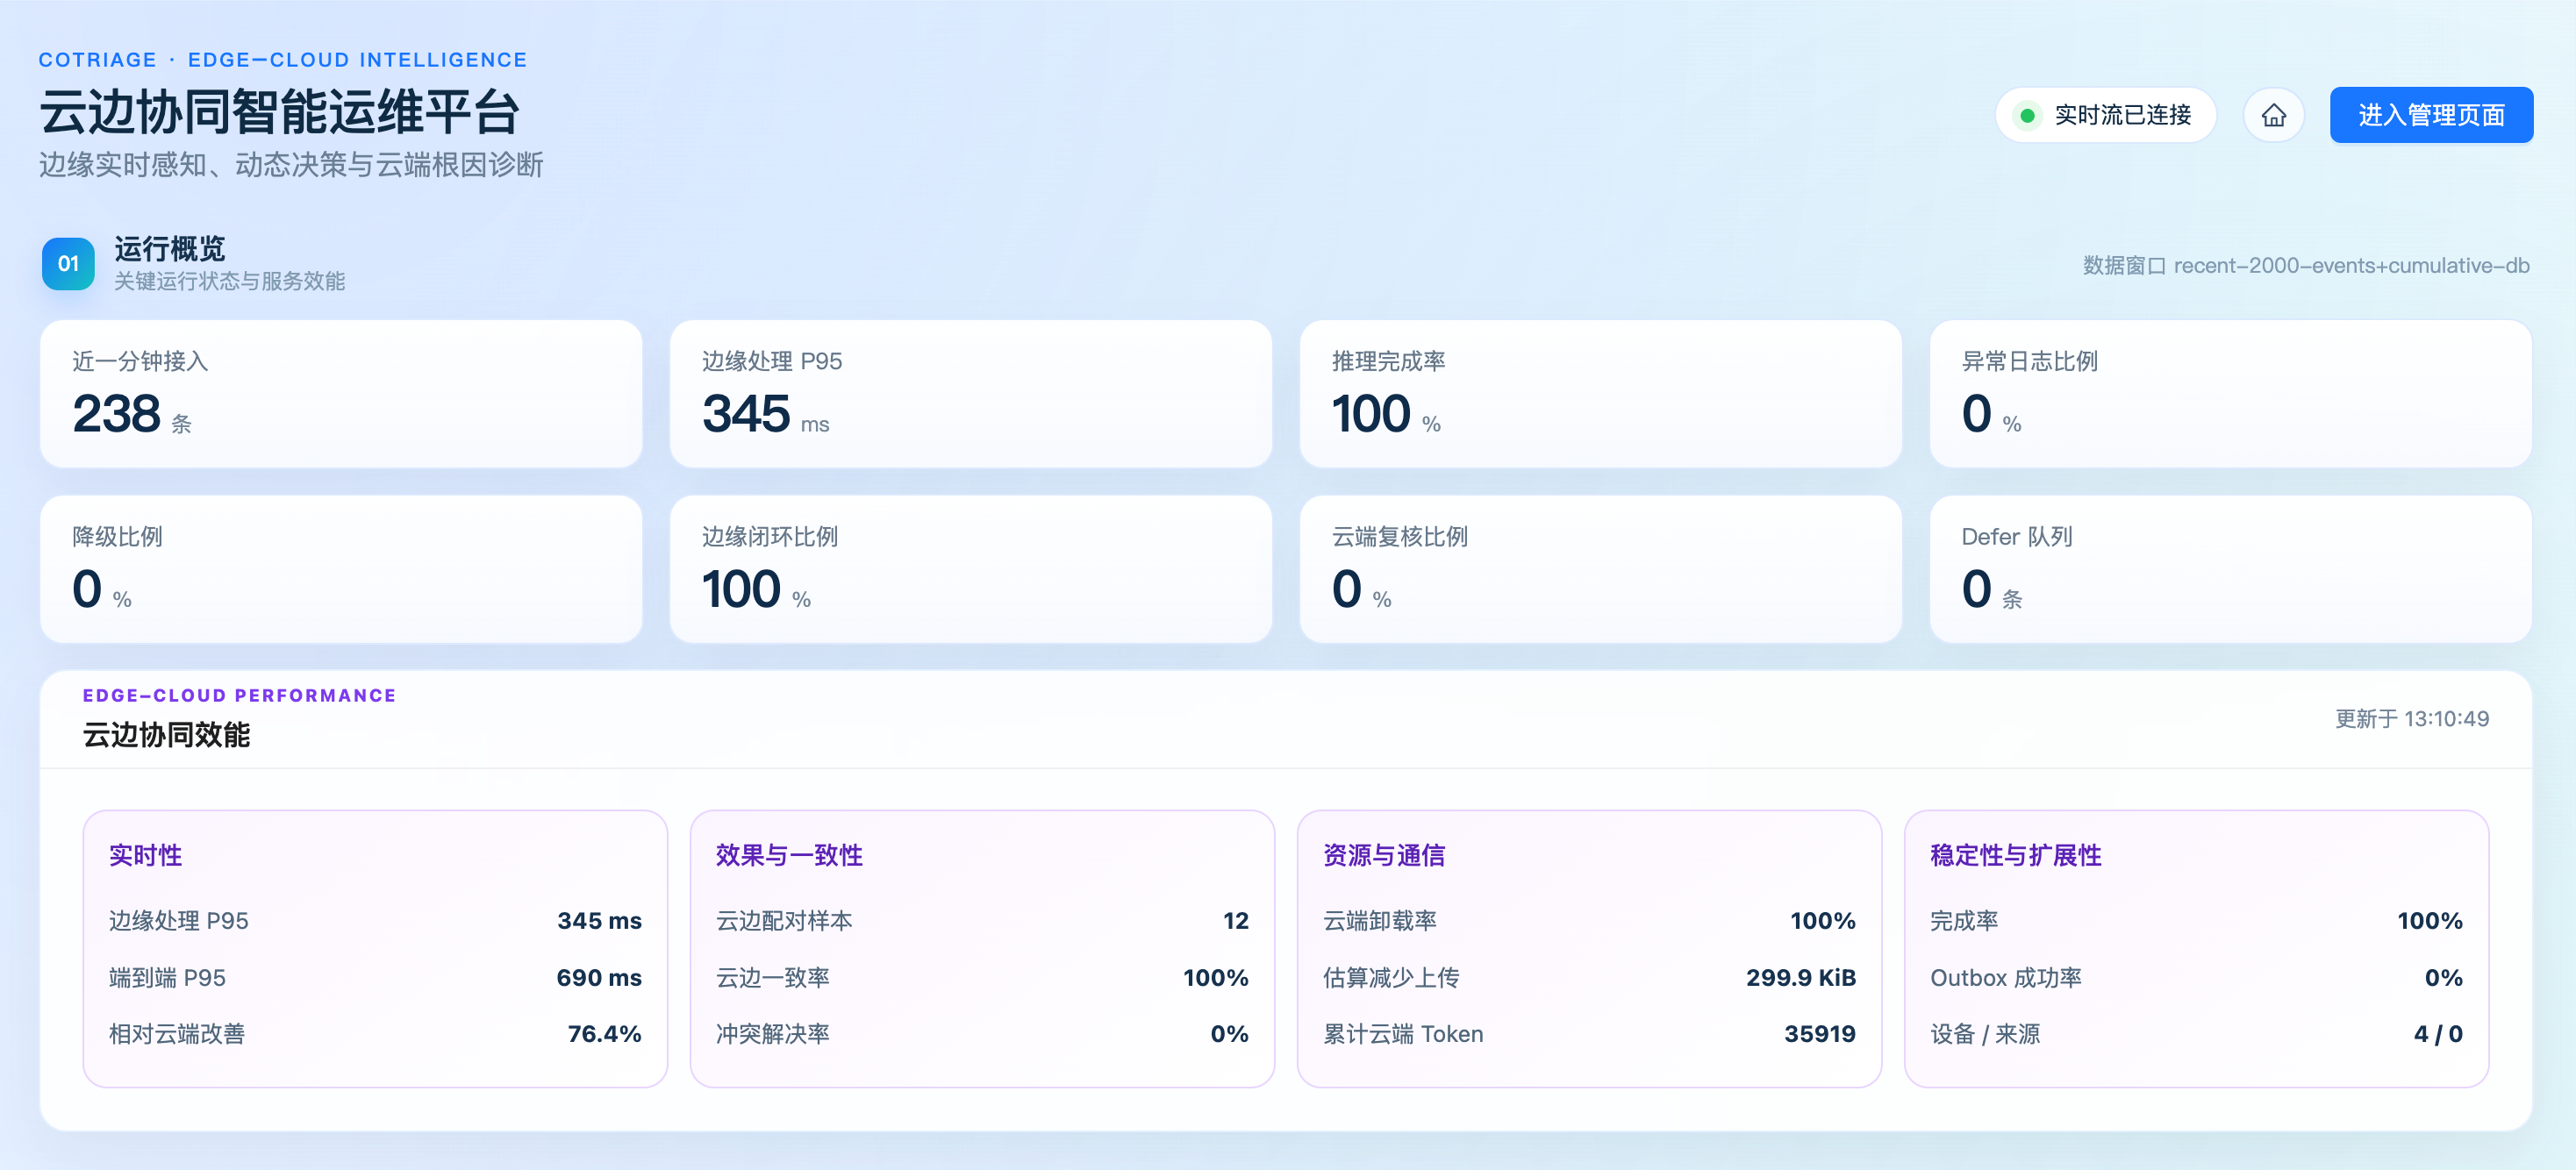
\includegraphics[width=\textwidth]{figures/s-11-competition-metrics-dashboard.png}
  \caption{运行看板样张}
\end{figure}

\clearpage
\printbibliography[heading=bibintoc,title={参考文献}]
\end{document}
